\chapter{Additional Images}~\label{ch:additionalImages}

\begin{figure}[ht]
    \centering
    % Subfigure for textual description
    \begin{subfigure}[b]{0.20\textwidth}
        \centering
        \fontsize{9pt}{7pt}\selectfont\text{Iteration = 100}\vspace{3cm}
        \fontsize{9pt}{7pt}\selectfont\text{Iteration = 5000}\vspace{2.85cm}
        \fontsize{9pt}{7pt}\selectfont\text{Iteration = 10000}\vspace{1.95cm}
    \end{subfigure}
    \begin{subfigure}[b]{0.20\textwidth}
        \centering
        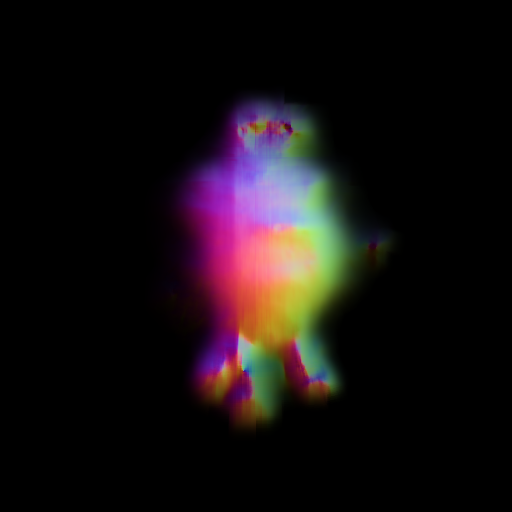
\includegraphics[width=\textwidth]{etc/a robot made out of plants/dreamfusion2/dreamfusion_plantrobot_1_part2.png}
        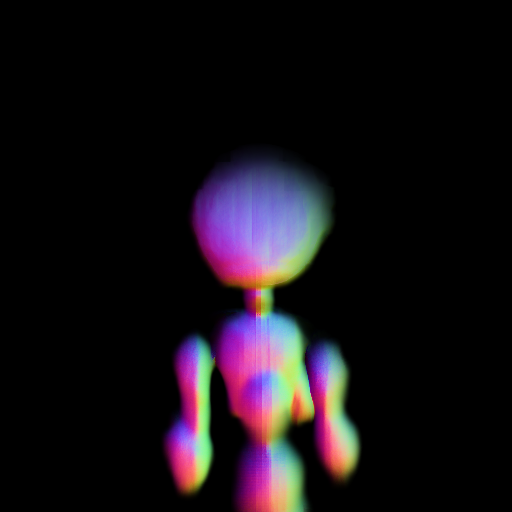
\includegraphics[width=\textwidth]{etc/a robot made out of plants/dreamfusion2/dreamfusion_plantrobot_5000_part2.png}
        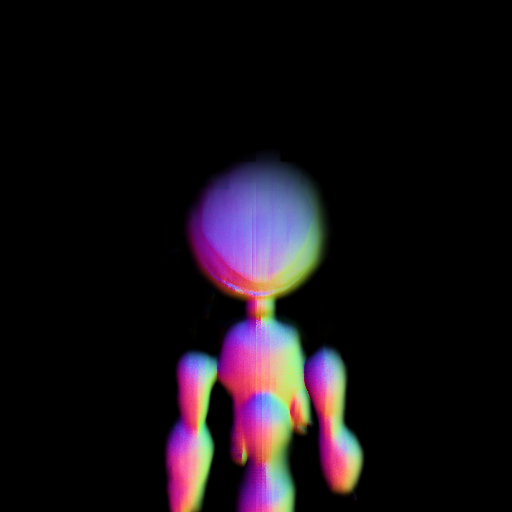
\includegraphics[width=\textwidth]{etc/a robot made out of plants/dreamfusion2/dreamfusion_plantrobot_10000_part2.png}
        \caption{}
    \end{subfigure}
    \begin{subfigure}[b]{0.20\textwidth}
        \centering
        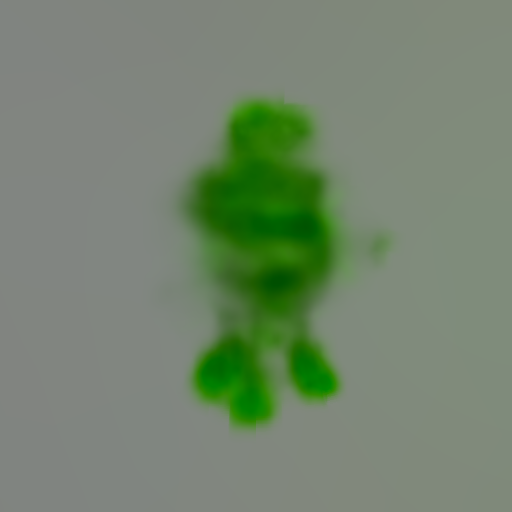
\includegraphics[width=\textwidth]{etc/a robot made out of plants/dreamfusion2/dreamfusion_plantrobot_1_part1.png}
        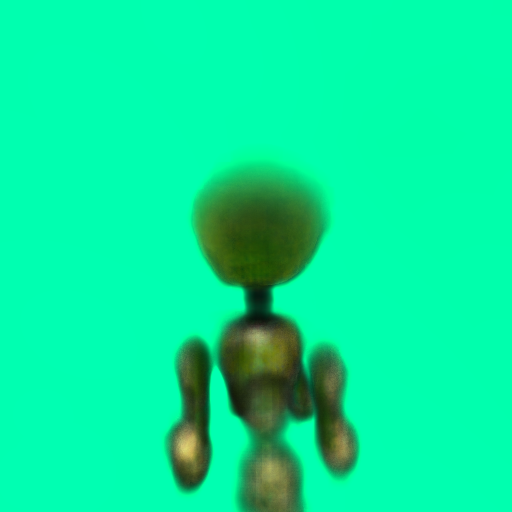
\includegraphics[width=\textwidth]{etc/a robot made out of plants/dreamfusion2/dreamfusion_plantrobot_5000_part1.png}
        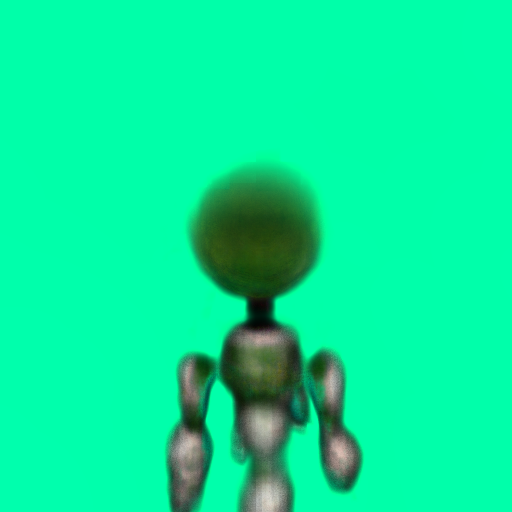
\includegraphics[width=\textwidth]{etc/a robot made out of plants/dreamfusion2/dreamfusion_plantrobot_10000_part1.png}
        \caption{}
    \end{subfigure}
    % Subfigure 3
    \hspace{.5cm}
    \begin{subfigure}[b]{0.252\textwidth}
        \centering
        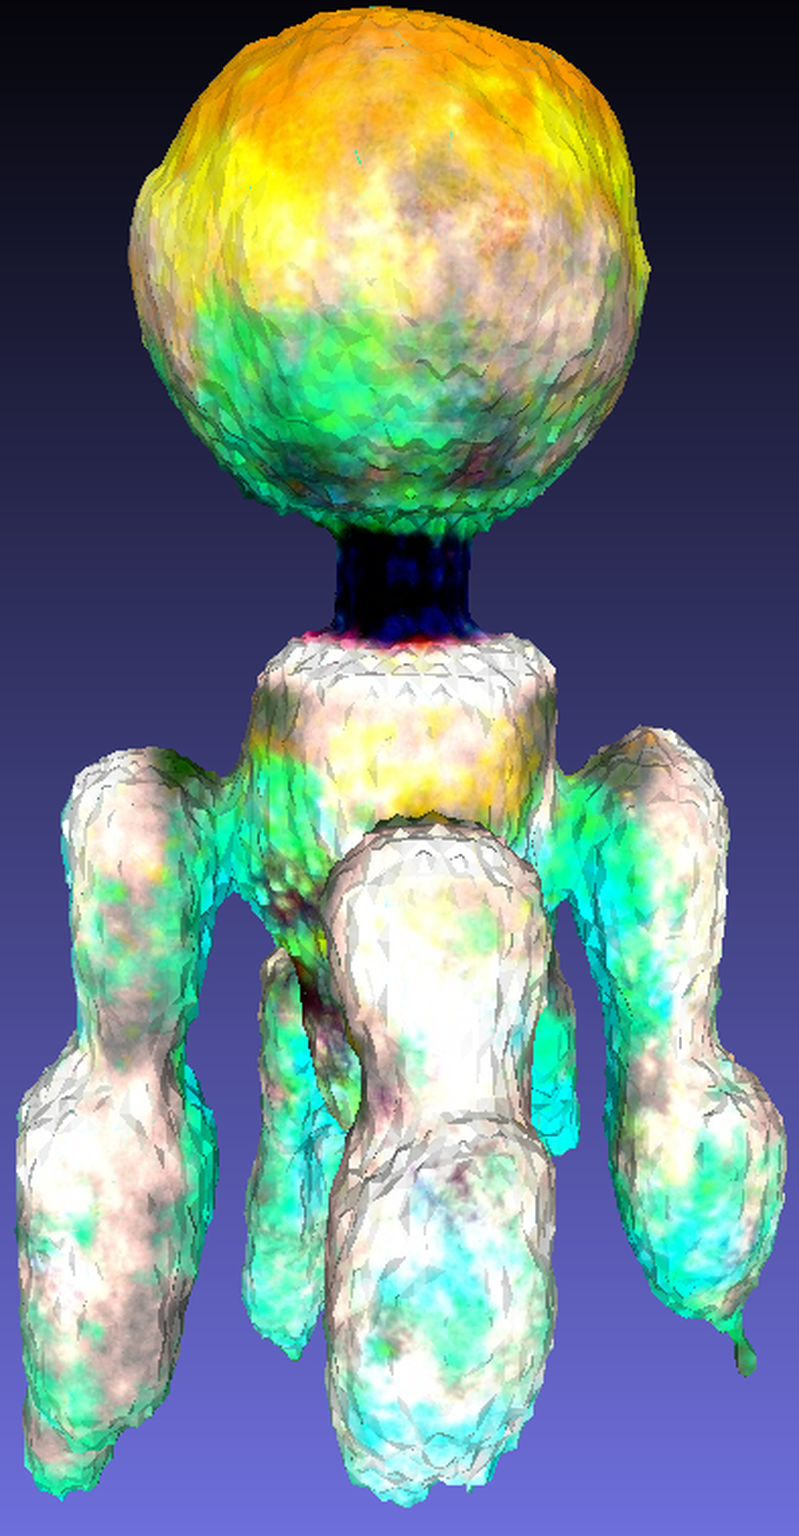
\includegraphics[width=\textwidth]{etc/a robot made out of plants/dreamfusion2/dreamfusion_plantrobot_model_resized.png}
        \caption{}
    \end{subfigure}
    \caption{The generation process of DreamFusion using the prompt ``a robot made out of plants'' a second time.}~\label{fig:secondRobotDreamfusion}
\end{figure}


\begin{figure}[ht]
    \centering
    % Subfigure for textual description
    \begin{subfigure}[b]{0.20\textwidth}
        \centering
        \fontsize{9pt}{7pt}\selectfont\text{Iteration = 0}\vspace{3cm}
        \fontsize{9pt}{7pt}\selectfont\text{Iteration = 5000}\vspace{2.85cm}
        \fontsize{9pt}{7pt}\selectfont\text{Iteration = 10000}\vspace{1.95cm}
    \end{subfigure}
    \begin{subfigure}[b]{0.20\textwidth}
        \centering
        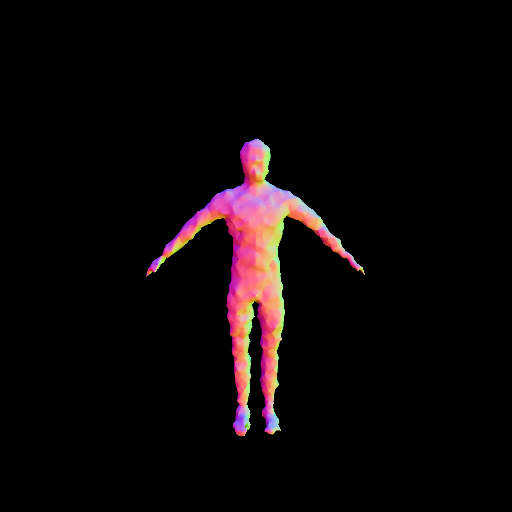
\includegraphics[width=\textwidth]{etc/a robot made out of plants/fantasia3d_fromMesh/fantasia_coarse_robot_0_part2.png}
        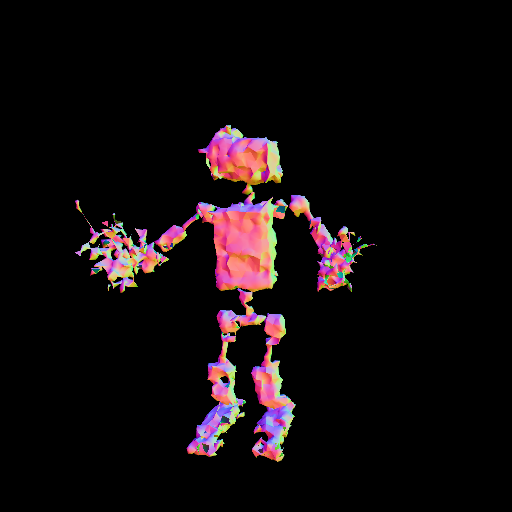
\includegraphics[width=\textwidth]{etc/a robot made out of plants/fantasia3d_fromMesh/fantasia_coarse_robot_5000_part2.png}
        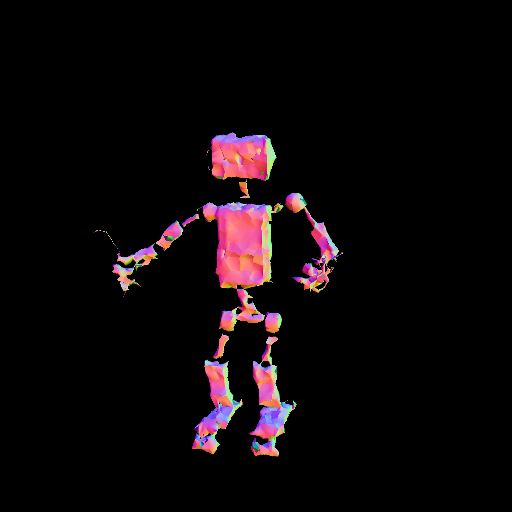
\includegraphics[width=\textwidth]{etc/a robot made out of plants/fantasia3d_fromMesh/fantasia_coarse_robot_10000_part2.png}
        \caption{}
    \end{subfigure}
    \begin{subfigure}[b]{0.20\textwidth}
        \centering
        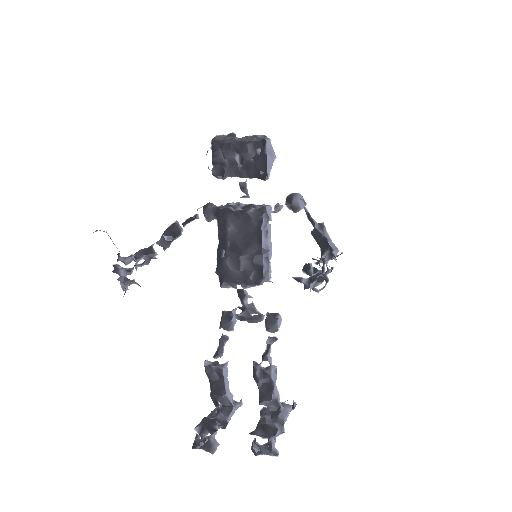
\includegraphics[width=\textwidth]{etc/a robot made out of plants/fantasia3d_fromMesh/fantasia_refine_robot_0_part1.png}
        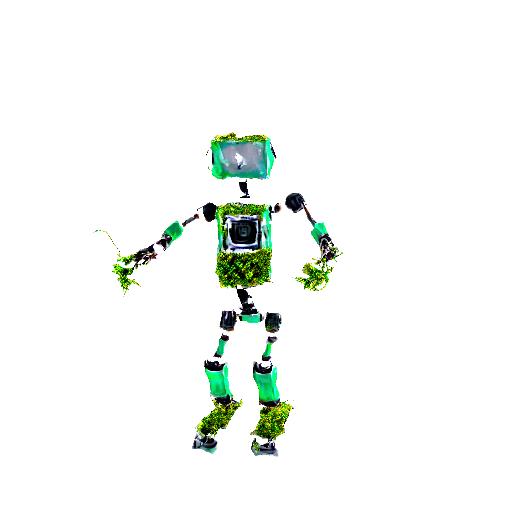
\includegraphics[width=\textwidth]{etc/a robot made out of plants/fantasia3d_fromMesh/fantasia_refine_robot_5000_part1.png}
        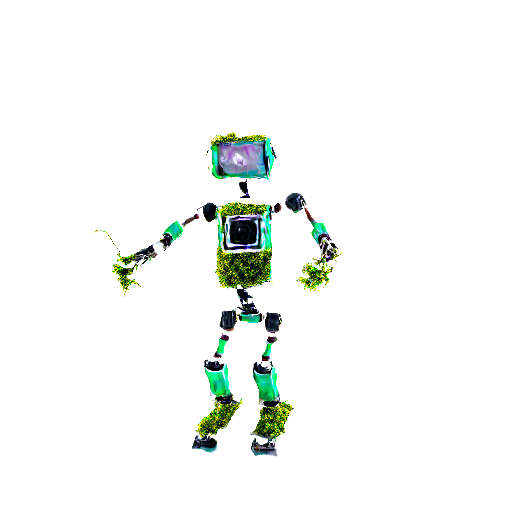
\includegraphics[width=\textwidth]{etc/a robot made out of plants/fantasia3d_fromMesh/fantasia_refine_robot_10000_part1.png}
        \caption{}
    \end{subfigure}
    % Subfigure 3
    \begin{subfigure}[b]{0.37\textwidth}
        \centering
        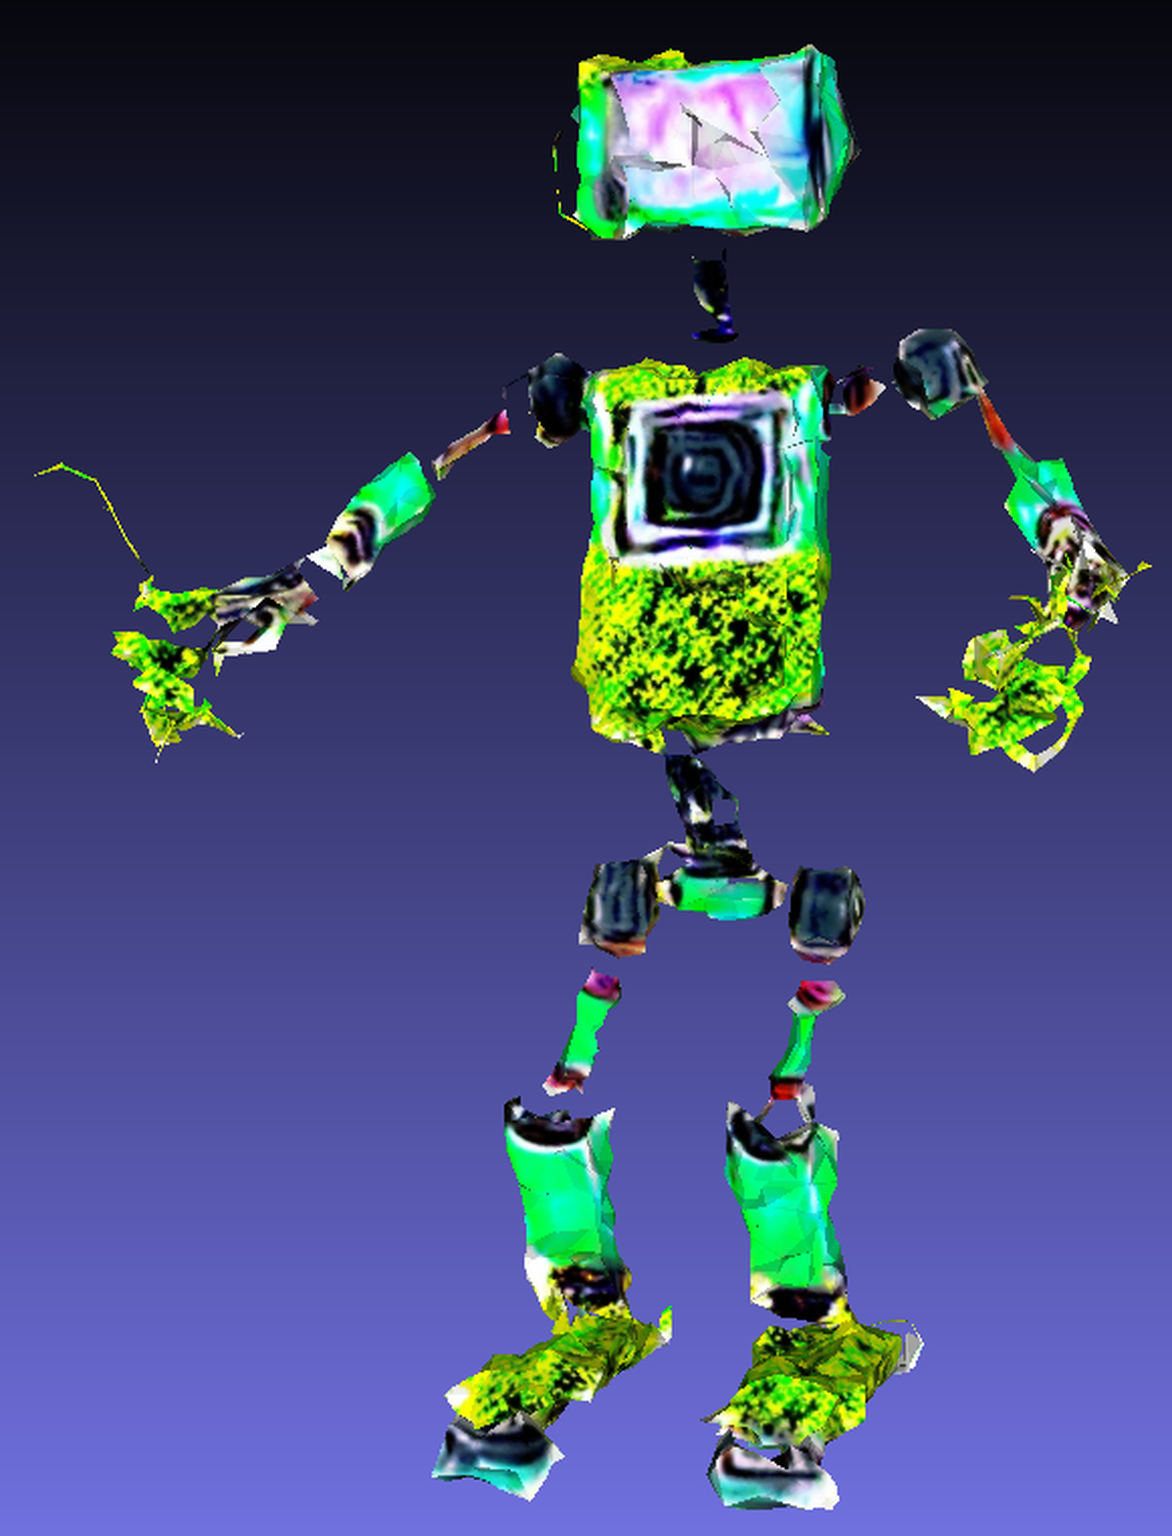
\includegraphics[width=\textwidth]{etc/a robot made out of plants/fantasia3d_fromMesh/fantasia_plantrobot_model_resized.png}
        \caption{}
    \end{subfigure}
    \caption{Initializing Fantasia3D with a coarse mesh representing a basic human figure}~\label{fig:generationFantasia2}
\end{figure}